\documentclass[letterpaper]{article}
\usepackage{flairs}%aaai
\usepackage{times}
\usepackage{helvet}
\usepackage{courier}
\usepackage{graphicx}
\usepackage{setspace}
\usepackage{url}
\frenchspacing
\setlength{\pdfpagewidth}{8.5in}
\setlength{\pdfpageheight}{11in}
\pdfinfo{
/Title (The Interactive Interpretation Viewer)
/Author (Jack McKeown, Geoff Sutcliffe)} 

\setcounter{secnumdepth}{2}  

%----Making things more compact
\newcommand{\smalltt}[1]{\small \texttt{#1}}
\newenvironment{packed_itemize}{
\vspace*{-0.2em}
\begin{itemize}
\setlength{\partopsep}{0pt}
\setlength{\itemsep}{1pt}
\setlength{\parskip}{0pt}
\setlength{\parsep}{0pt}
}{\end{itemize}}
\newenvironment{packed_enumerate}{
\vspace*{-0.2em}
\begin{enumerate}
\setlength{\partopsep}{0pt}
\setlength{\itemsep}{1pt}
\setlength{\parskip}{0pt}
\setlength{\parsep}{0pt}
}{\end{enumerate}}
\renewcommand{\textfraction}{0.07}
\renewcommand{\topfraction}{0.9}
\renewcommand{\bottomfraction}{0.9}
\renewcommand{\floatpagefraction}{0.66}
\setlength{\floatsep}{2.0pt plus 2.0pt minus 2.0pt}
\setlength{\textfloatsep}{10.0pt plus 2.0pt minus 0.0pt}

\begin{document}

\title{An Interactive Interpretation Viewer for Typed First-order Logic}
\author{Jack McKeown\\
University of Miami\\
USA\\
\And
Geoff Sutcliffe\\
University of Miami\\
USA}

\maketitle
% \begin{abstract}
% \begin{quote}
% This poster describes the Interactive Interpretation Viewer - IIV, for finite interpretations 
% in typed first-order logic written in the (new) TPTP format for interpretations.
% \end{quote}
% \end{abstract}
%--------------------------------------------------------------------------------------------------
\section{Introduction}
\label{Introduction}

Historically, Automated Theorem Proving (ATP) has, as the name suggests, focused largely on the 
task of proving theorems from axioms -- the derivation of conclusions that follow inevitably from 
known facts \cite{RV01-HAR}.
The axioms and conjecture to be proved (to become a theorem) are written in an 
appropriately expressive logic, and the proofs are often similarly written in logic \cite{SS+06}.
In the last two decades the converse task of disproving conjectures has become increasingly 
important.
This is achieved by finding an {\em interpretation} -- a structure that maps terms to domain 
elements and formulae to truth values, that is a {\em model} of the axioms -- it maps the axioms to 
{\em true}, and a {\em countermodel} of the conjecture -- it maps the conjecture to {\em false}
(or equivalently, it is a model of the negated conjecture).
% A conjecture is disproved by finding an interpretation that is a model of the axioms, but 
% it maps the conjecture to {\em false}.
A salient application area that harnesses this form of ATP is verification \cite{DKW08}.
% where a countermodel is used to pinpoint the reason why a proof obligation fails, and
% correspondingly points to the location of the fault in the system being verified.
This work describes an interactive interpretation viewer for finite interpretations 
written in the (new) TPTP format for interpretations \cite{SS+22-FLAIRS}, for formulae in
typed first-order logic.

% \paragraph{Related Work:}
% Related work is sparse.
% The Mace4 model finder \cite{McC03-MACE4-TR} outputs textual 
% information about the models it finds, including the interpretation of constants as integers,
% and tables for the function and predicate symbols' interpretations. 
% The tables are naturally limited to symbols of arity up to two (which is just fine for algebras, 
% where Mace4 is often applied).
% The only graphical visualization tool that has been found is that described in \cite{Sch13-MS},
% which provided (past tense -- it is no longer available) a visualization of finite first-order 
% interpretations as produced by Paradox.
% The visualization had some nice features, e.g., showing functions as constructor functions, and 
% reducing the visual clutter when displaying relations with properties such as symmetry, 
% transitivity, etc.
% In other ways that work was quite different from the visualization described in this work.

%--------------------------------------------------------------------------------------------------
\section{The TPTP World and Languages}
\label{TPTP}

The TPTP World \cite{Sut17} is a well established infrastructure that supports research, 
development, and deployment of ATP systems.
The TPTP language \cite{Sut22-IGPL} is 
% one of the keys to the success of the TPTP World.
% The language is 
used for writing both problems and solutions (derivations and interpretations).
The top level building blocks of the TPTP language are {\em annotated formulae}.
An annotated formula has the form:\\
\hspace*{0.5cm}{\em language}{\tt (}{\em name}{\tt ,}
{\em role}{\tt ,}
{\em formula}{\tt ,}
{\em source}{\tt ,}
{\em useful\_info}{\tt )}\\
The {\em language}s supported are {\smalltt{cnf}} (clause normal form), {\smalltt{tcf}} (typed
clause normal form), {\smalltt{fof}} (first-order form), {\smalltt{tff}} (typed first-order form), 
and {\smalltt{thf}} (typed higher-order form).
The {\em role}, e.g., {\smalltt{type}}, {\smalltt{axiom}}, {\smalltt{conjecture}}, defines the use 
of the formula in an ATP system.
The {\em formula} follows Prolog conventions, and can
% -- functions and predicates start with a lowercase letter or are {\tt '}single quoted{\tt '}, and 
% variables start with an uppercase letter.
additionally include interpreted symbols that start with a {\tt \$}, e.g., {\smalltt{\$true} and
its boolean type {\smalltt{\$o}}.
% and {\smalltt{\$false}}, 
% and numbers.
% integer/rational/real numbers such as 27, 43/92, -99.66.
The logical connectives are
{\tt !}, {\tt ?}, {\tt \verb|~|}, {\tt |}, {\tt \&}, {\tt =>}, {\tt <=}, {\tt <=>}, and 
{\tt <{\raisebox{0.4ex}{\texttildelow}}>}.
for
$\forall$, $\exists$, $\neg$, $\vee$, $\wedge$, $\Rightarrow$, $\Leftarrow$, $\Leftrightarrow$, 
and $\oplus$ respectively.
Equality and inequality are expressed as the infix operators {\tt =} and {\tt !=}.
The {\em source} and {\em useful\_info} are optional.
Figure~\ref{TF0FiniteProblem} is an example of a problem (not a theorem!) in monomorphic 
typed first-order form (TF0).  
% The associated (counter)model is discussed in Section~\ref{Interpretations}.

\begin{figure}[htbp]
\scriptsize
\setstretch{0.8}
\begin{verbatim}
%--------------------------------------------------------
tff(human_type,type,      human: $tType ).
tff(cat_type,type,        cat: $tType ).
tff(jon_decl,type,        jon: human ).
tff(garfield_decl,type,   garfield: cat ).
tff(arlene_decl,type,     arlene: cat ).
tff(nermal_decl,type,     nermal: cat ).
tff(loves_decl,type,      loves: cat > cat ).
tff(owns_decl,type,       owns: ( human * cat ) > $o ).

tff(three_cats,axiom,
    $distinct(garfield,arlene,nermal) ).

tff(jon_owns_garfield_not_arlene,axiom,
    ( owns(jon,garfield) & ~ owns(jon,arlene) ) ).

tff(all_cats_love_garfield,axiom,
    ! [C: cat] : ( loves(C) = garfield ) ).

tff(jon_owns_garfields_lovers,conjecture,
    ! [C: cat] :
      ( ( loves(C) = garfield & C != arlene ) 
     => owns(jon,C) ) ).
%--------------------------------------------------------
\end{verbatim}
\caption{A TF0 problem
% (with a finite countermodel)
% \\
% {\scriptsize \url{https://raw.githubusercontent.com/GeoffsPapers/IIVPoster/main/TFF_Finite.p}}
}
\label{TF0FiniteProblem}
\end{figure}

%--------------------------------------------------------------------------------------------------
\section{Interpretations}
\label{Interpretations}

A Tarskian-style interpretation \cite{TV56} of formulae in typed first-order logic consists of a 
non-empty domain of unequal elements for each type (just one domain for untyped logic), and 
interpretations of the function and predicate symbols with respect to the domains 
\cite{Gal15}.
Interpretations with only finite domains are called {\em finite interpretations}, and
interpretations with one of more infinite domains are called {\em infinite interpretations}.
Finite domains are commonly explicitly enumerated, but can also take other forms, e.g., the 
finite Herbrand Universe of a Herbrand interpretation \cite{Her30}.
This work deals with only enumerated finite domains.
% Infinite domains can take several forms, including being implicitly specified (e.g., some set
% of algebraic numbers, such as the integers), explicitly generated (e.g., terms representing 
% Peano numbers), and the infinite Herbrand Universe of a Herbrand interpretation.
The TPTP representation of an interpretation uses an {\em interpretation formula}, preceded by 
the necessary type declarations.
%\begin{packed_itemize}
%\item the type declarations for the formulae being interpreted;
%\item the types of the domains (unless already defined in the language, e.g., the type
%      {\smalltt{\$int}});
%\item the types of type-promotion functions from the types of the domains to the types 
%      of the formulae, used to make the interpretation formula well-typed;
%\item the types of the domain elements.
%\end{packed_itemize}
% \vspace*{-0.4em}
The interpretation formula is a conjunction providing details of the domains - their types and 
elements, and the interpretation of the symbols applied to domain elements.
Type-promotion functions are used to convert domain elements to terms, to make the
interpretation formula well-typed.
% \begin{packed_itemize}
% \item for each type in the formulae:
%       \begin{packed_itemize}
%       \item the domain type, by a formula that makes the type-promotion function a surjection;
%       \item the domain elements as a universally quantified disjunction of equalities whose 
%             right-hand sides are the domain elements;
%       \item specification of the distinctness of the domain elements;
%       \item a formula making the type-promotion function an injection,
%             which with the surjectivity makes it a bijection.
%       \end{packed_itemize}
% \item interpretation of the function symbols, as equalities whose left-hand sides are 
%       formed from symbols applied to type-promoted domain elements, and whose right-hand sides 
%       are type-promoted domain elements;
% \item interpretation of the predicate symbols, as literals formed from symbols applied
%       to type-promoted domain elements; positive literals are {\em true} and negative literals 
%       are {\em false}.
% \end{packed_itemize}
The representation is also usable for untyped first-order logic, where all terms in both the 
given and interpretation formulae are of the same type -- ``individuals''., which obviates the 
need for type considerations, in particular type-promotion functions are not needed.
 
Figure~\ref{TF0FiniteInterpretation} is a TF0 interpretation with finite domains -- it is a 
countermodel for the problem in Figure~\ref{TF0FiniteProblem}.
The type declarations have been omitted, and can be found in the URL provided.
% The comments show which parts of the formula specify what aspects of the interpretation, per
% the list above.

\begin{figure}[htbp]
\scriptsize
\setstretch{0.8}
\begin{verbatim}
%--------------------------------------------------------
tff(garfield,interpretation,
%----The domain for human
    ( ( ! [H: human] : ? [DH: d_human] : H = d2human(DH)
      & ! [DH: d_human] : ( DH = d_jon )
      & ! [DH1: d_human,DH2: d_human] :
          ( d2human(DH1) = d2human(DH2) => DH1 = DH2 )
%----The domain for cat
      & ! [C: cat] : ? [DC: d_cat] : C = d2cat(DC)
      & ! [DC: d_cat]: ( DC = d_garfield | DC = d_arlene )
      & $distinct(d_garfield,d_arlene,d_nermal)
      & ! [DC1: d_cat,DC2: d_cat] :
          ( d2cat(DC1) = d2cat(DC2) => DC1 = DC2 ) )
%----Interpret terms and atoms
    & ( jon = d2human(d_jon)
      & garfield = d2cat(d_garfield)
      & arlene = d2cat(d_arlene)
      & nermal = d2cat(d_nermal)
      & loves(d2cat(d_garfield)) = d2cat(d_garfield)
      & loves(d2cat(d_arlene)) = d2cat(d_garfield)
      & loves(d2cat(d_nermal)) = d2cat(d_garfield) )
    & ( owns(d2human(d_jon),d2cat(d_garfield))
      & ~ owns(d2human(d_jon),d2cat(d_arlene))
      & ~ owns(d2human(d_jon),d2cat(d_nermal)) ) ) ).
%--------------------------------------------------------
\end{verbatim}
\caption{A TF0 countermodel for the problem in Figure~\ref{TF0FiniteProblem} \\
{\scriptsize \url{https://raw.githubusercontent.com/GeoffsPapers/IIVPoster/main/TFF_Finite.s}}}
\label{TF0FiniteInterpretation}
\end{figure}

%--------------------------------------------------------------------------------------------------
\section{Interpretation Visualization}
\label{Visualization}

Proof visualization is well-established, with several tools available, including the Interactive 
Derivation Viewer (IDV) -- a tool for visualizing TPTP format proofs \cite{TPS07}.
Interpretation visualization, however, has (to the knowledge of the authors) had minimal 
attention, with \cite{Sch13-MS} being the only tool found (past tense -- it is no longer
available).
Visualization of interpretations is useful in areas such as teaching logic, debugging ATP 
systems, and understanding a model.
A visualization for TF0 interpretations has been designed in this work,
% and the initial implementation 
and it is available as the IIV tool in the SystemOnTSTP web interface\footnote{%
\url{https://www.tptp.org/cgi-bin/SystemOnTSTP}}.
% The implementation is ``initial'' because it is fully automated only for finite TF0 and untyped
% logic interpretations.
% ; for infinite interpretations different components of the interpretation formula 
% have to be manually extracted into separate annotated formulae, to mimic a derivation that IDV 
% can render.

Figure~\ref{TF0FiniteIIV} is the visualization of the interpretation in 
Figure~\ref{TF0FiniteInterpretation}.
The top row of inverted triangles are the types in the problem formulae,
while the bottom row of inverted triangles are the types of the domains in the interpretation
formula.
The inverted houses are the function and predicate symbols, and the successive rows of ovals are 
the successive domain element arguments used in the symbols' interpretations.
Finally, the row of houses and boxes are the interpretations of the symbols applied to those
arguments; houses for functions and boxes for predicates.
Paths from leaf to root nodes show the interpretations of the symbols applied to the 
domain elements.
For example, in the given formulae the type of {\smalltt{loves}} is {\smalltt{cat}},
and {\smalltt{loves(d\_arlene)}} is interpreted as {\smalltt{d\_garfield}}, which is of type
{\smalltt{d\_cat}} in the interpretation formula.
% Similarly, in the given formulae the type of {\smalltt{owns}} is {\smalltt{\$o}}, and
% {\smalltt{owns(d\_jon,d\_garfield)}} is interpreted as {\smalltt{\$true}}, which is of type
% {\smalltt{\$o}} in the interpretation formula.

IIV provides some interactive features: Figure~\ref{TF0FiniteIIV} shows the situation with the 
cursor hovering over the {\smalltt{d\_garfield}} node on the path from {\smalltt{owns}} to 
{\smalltt{\$true}}, showing that {\smalltt{owns(d\_jon,d\_garfield)}} is interpreted as 
{\smalltt{\$true}}.
The nodes above are increasingly darker red (grey if printed) up to the type node {\smalltt{\$o}} 
that is the result type of {\smalltt{owns}}, and increasingly darker blue down to the type node 
{\smalltt{\$o}} that is the type of {\smalltt{\$true}}.
This highlighting provides easy focus on the interpretations of chosen symbols, e.g., it is easy
to highlight what symbol applications are interpreted as {\smalltt{\$true}} or {\smalltt{\$false}}
by hovering over the corresponding truth value node, or how a specific function symbol is 
interpreted, e.g, by hovering over the {\smalltt{loves}} node.

This visualization is available in IIV using the URL provided with 
Figure~\ref{TF0FiniteInterpretation} as the ``URL to fetch from'',
selecting {\tt IIV 0.0} as the ``System'', and clicking the ``Process Solution'' button.

\begin{figure}[htbp]
\centering
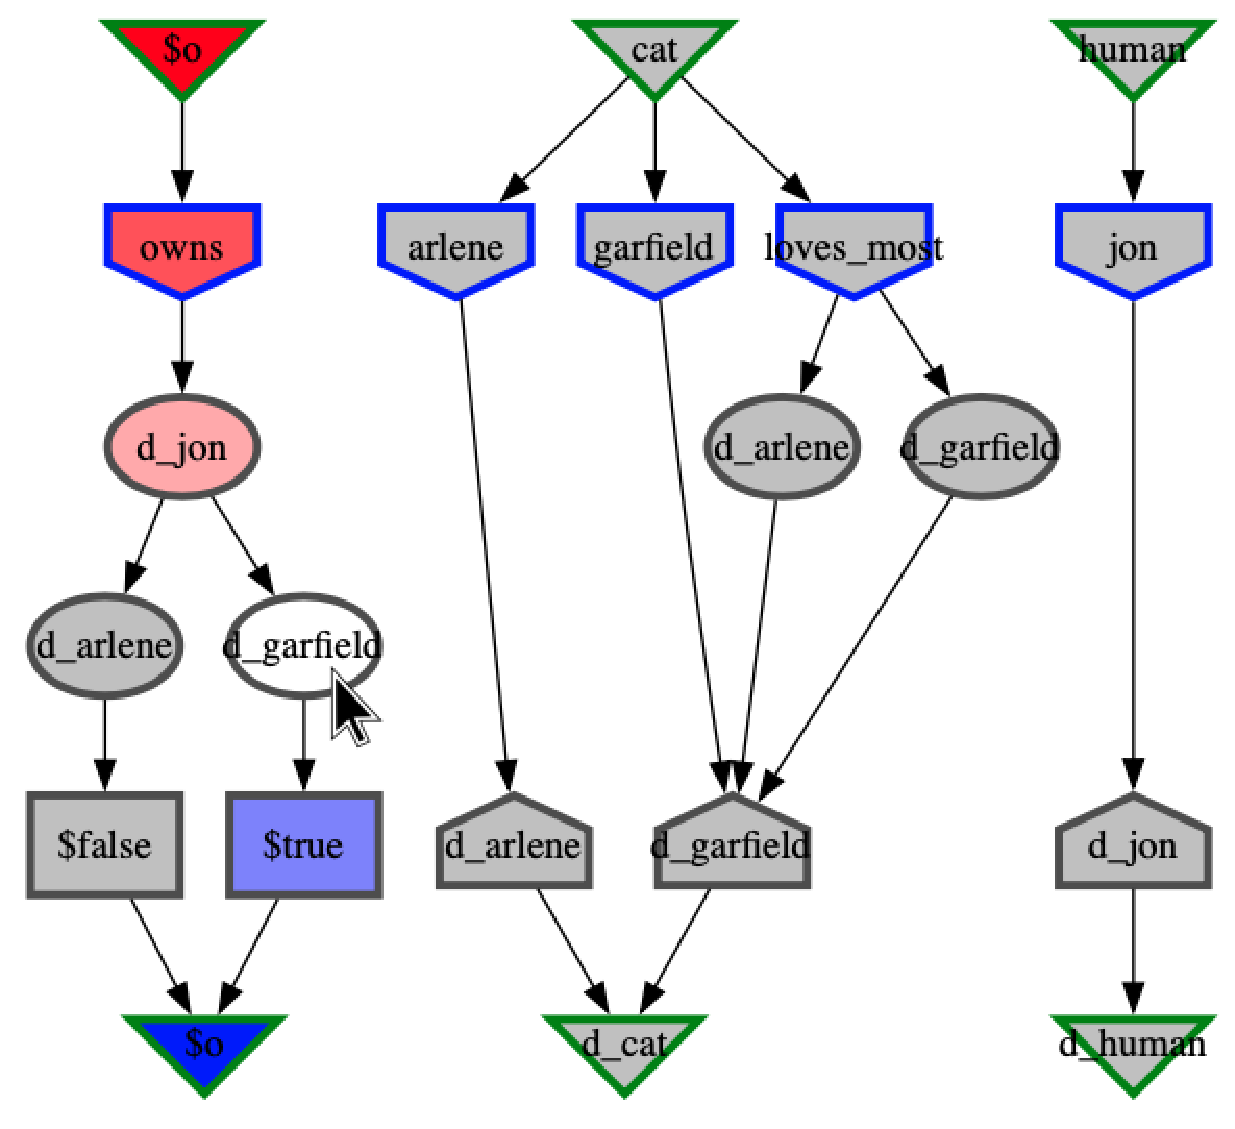
\includegraphics[width=\columnwidth]{IIVGraph.pdf}
\caption{Visualization of the interpretation in Figure~\ref{TF0FiniteInterpretation}}
\label{TF0FiniteIIV}
\end{figure}

%--------------------------------------------------------------------------------------------------
\section{IIV Implementation}
\label{Implementation}

IIV is implemented on top of IDV, and has benefited from the mature state of IDV.
Different terms in an interpretation, e.g., problem types, problem symbols, domain elements,
domain types, are extracted into annotated formulae with different languages and roles that
IDV renders differently: 
types are extracted into {\smalltt{fof}} annotated formulae with the role {\smalltt{axiom}}
that are rendered as inverted triangles with a green outline;
problem symbols are extracted into {\smalltt{thf}} {\smalltt{negated\_conjecture}}s
that are rendered as inverted houses with a blue outline;
domain element arguments for problem symbols are extracted into {\smalltt{tcf}} {\smalltt{plain}}s
that are rendered as ellipses with a grey outline;
domain element interpretations for function symbols are extracted into {\smalltt{tcf}}
{\smalltt{conjecture}}s that are rendered as houses with a grey outline;
truth value interpretations for predicate symbols are extracted into {\smalltt{tcf}}
{\smalltt{conjecture}}s that are rendered as boxes (as a special case) with a grey outline.
A ``derivation'' is formed by setting the ``inference'' parents of each node appropriately.
%  e.g., problem symbols are extracted into annotated formulae with
% the language {\smalltt{thf}} and the role {\smalltt{negated\_conjecture}}, which IDV renders 
% as inverted houses with a blue outline.
% which IDV renders as the directed links between nodes.
In order to separate nodes for different kinds of terms into different layers, a {\smalltt{level}}
term is added to the source field of each derivation annotated formula, which is used by IDV only
when rendering interpretations.

A Prolog program is used to extract the components of the interpretation formulae into 
the separate derivation annotated formulae.
ANTLR is used to generate a JavaScript parser for the TPTP language.
The parser is used in the browser, along with custom JavaScript, to create a graph in 
the Graphviz DOT language \cite{EG+02} from the TPTP input (in this case, representing an 
interpretation).
The resulting DOT text is then rendered using the ``d3-graphviz''\footnote{%
\url{https://github.com/magjac/d3-graphviz}} library, which uses WebAssembly for speed.

% \begin{packed_itemize}
% \item each problem type is extracted into a {\smalltt{fof}} annotated formula with the role 
%       {\smalltt{axiom}}, which is rendered as an inverted triangle with a green outline;
% \item each problem symbol is extracted into a {\smalltt{thf}} {\smalltt{negated\_conjecture}}
%       whose parent (as an IDV inference) is annotated formula containing the symbol's type,
%       and is rendered as an inverted house with a blue outline;
% \item each domain element argument in the interpretation of a symbol is extracted into a
%       {\smalltt{tcf}} {\smalltt{plain}} annotated formula whose parents are either annotated
%       formulae for symbols or the annotated formula for the preceding argument,
%       and is rendered as an ellipse with a grey outline;
% \item each domain element interpretation for function symbols is extracted into a {\smalltt{tcf}} 
%       {\smalltt{conjecture}} whose parents are the last annotated formulae of paths from symbols 
%       through domain elements,
%       and is rendered as a house with a grey outline;
% \item each truth value interpretation for predicate symbols is extracted into a {\smalltt{tcf}} 
%       {\smalltt{conjecture}} whose parents are the last annotated formulae of paths from symbols
%       through domain elements,
%       and is rendered as a box (as a special case) with a grey outline;
% \end{packed_itemize}

%--------------------------------------------------------------------------------------------------
\section{Future Work}
\label{Future}

Further inspiration might lead to improvements to IDV, especially for infinite interpretations
and Kripke interpretations \cite{Kri63} for non-classical logics.

%--------------------------------------------------------------------------------------------------
\bibliographystyle{flairs}
\bibliography{Bibliography.bib}
%--------------------------------------------------------------------------------------------------
\end{document}
%--------------------------------------------------------------------------------------------------
%% \section{Formatting Requirements in Brief}
%% We need source and PDF files that can be used in a variety of ways and can be output on a variety of devices. FLAIRS imposes some requirements on your source and PDF files that must be followed. Most of these requirements are based on our efforts to standardize conference manuscript properties and layout. These requirements are as follows, and all papers submitted to FLAIRS for publication must comply:
%% 
%% \begin{itemize}
%% \item Your .tex file must compile in PDF\LaTeX{} --- \textbf{ no .ps or .eps figure files.}
%% \item All fonts must be embedded in the PDF file --- \textbf{ this includes your figures.}
%% \item Modifications to the style sheet (or your document) in an effort to avoid extra page  are NOT allowed.
%% \item No type 3 fonts may be used (even in illustrations).
%% \item Your title must follow US capitalization rules.
%% \item \LaTeX{} documents must use the Times or Nimbus font package (do not use Computer Modern for the text of your paper).
%% \item Fonts that require non-English language support (CID and Identity-H) must be converted to outlines or removed from the document (even if they are in a graphics file embedded in the document). 
%% \item Two-column format is required for all papers.
%% \item The paper size for final submission must be US letter. No exceptions.
%% \item The source file must exactly match the PDF.
%% \item The document margins must be as specified in the formatting instructions.
%% \item The number of pages and the file size must be as specified for your event.
%% \item No document may be password protected.
%% \item Neither the PDFs nor the source may contain any embedded links or bookmarks.
%% \item Your source and PDF must not have any page numbers, footers, or headers.
%% \item Your PDF must be compatible with Acrobat 5 or higher.
%% \item Your \LaTeX{} source file (excluding references) must consist of a \textbf{single} file (use of the ``input" command is not allowed.
%% \item Your graphics must be sized appropriately outside of \LaTeX{} (do not use the ``clip" command) .
%% \end{itemize}
%% 
%% If you do not follow the above requirements, it is likely that we will be unable to publish your paper.
%% 
%% \section{What Files to Submit}
%% You must submit the following items to ensure that your paper is published:
%% \begin{itemize}
%% \item A fully-compliant PDF file.
%% \item Your  \LaTeX{}  source file submitted as a \textbf{single} .tex file (do not use the ``input" command to include sections of your paper --- every section must be in the single source file). The only exception is the bibliography, which you may include separately. Your source must compile on our system, which includes the standard \LaTeX{} support files.
%% \item All your graphics files.
%% \item The \LaTeX{}-generated files (e.g. .aux and .bib file, etc.) for your compiled source.
%% \item All the nonstandard style files (ones not commonly found in standard \LaTeX{} installations) used in your document (including, for example, old algorithm style files). If in doubt, include it.
%% \end{itemize}
%% 
%% Your \LaTeX{} source will be reviewed and recompiled on our system (if it does not compile, you may incur late fees).   \textbf{Do not submit your source in multiple text files.} Your single \LaTeX{} source file must include all your text, your bibliography (formatted using flairs.bst), and any custom macros. Accompanying this source file, you must also supply any nonstandard (or older) referenced style files and all your referenced graphics files. 
%% 
%% Your files should work without any supporting files (other than the program itself) on any computer with a standard \LaTeX{} distribution. Place your PDF and source files in a single tar, zipped, gzipped, stuffed, or compressed archive. Name your source file with your last (family) name.
%% 
%% \textbf{Do not send files that are not actually used in the paper.} We don't want you to send us any files not needed for compiling your paper, including, for example, this instructions file, unused graphics files, and so forth.  
%% 
%% \section{Using \LaTeX{} to Format Your Paper}
%% 
%% The latest version of the FLAIRS style file is available on FLAIRS's website. Download this file and place it in a file named ``flairs.sty" in the \TeX\ search path. Placing it in the same directory as the paper should also work. You must download the latest version.
%% 
%% The following packages are incompatible with flairs.sty and/or flairs.bst and must not be used (this list is not exhaustive --- there are others as well):
%% \begin{itemize}
%% \item hyperref
%% \item natbib
%% \item geometry
%% \item titlesec
%% \item layout
%% \item caption
%% \item titlesec
%% \item T1 fontenc package (install the CM super fonts package instead)
%% \end{itemize}
%% 
%% \subsection{Illegal Commands}
%% The following commands may not be used in your paper:
%% \begin{itemize}
%% \item \textbackslash input
%% \item \textbackslash vspace (when used before or after a section or subsection)
%% \item \textbackslash addtolength 
%% \item \textbackslash columnsep
%% \item \textbackslash top margin (or text height or addsidemargin or even side margin)
%% \end{itemize}
%% 
%% \subsection{Paper Size, Margins, and Column Width}
%% Papers must be formatted to print in two-column format on 8.5 x 11 inch US letter-sized paper. The margins must be exactly as follows: 
%% \begin{itemize}
%% \item Top margin: .75 inches
%% \item Left margin: .75 inches
%% \item Right margin: .75 inches
%% \item Bottom margin: 1.25 inches
%% \end{itemize} 
%% 
%% 
%% The default paper size in most installations of \LaTeX{} is A4. However, because we require that your electronic paper be formatted in US letter size, you will need to alter the default for this paper to US letter size. Assuming you are using the 2e version of \LaTeX{}, you can do this by including the [letterpaper] option at the beginning of your file: 
%% \textbackslash documentclass[letterpaper]{article}. 
%% 
%% This command is usually sufficient to change the format. Sometimes, however, it may not work. Use PDF\LaTeX{} and include
%% \textbackslash setlength\{\textbackslash pdfpagewidth\}\{8.5in\}
%% \textbackslash setlength\{\textbackslash pdfpageheight\}\{11in\}
%% in your preamble. 
%% 
%% \textbf{Do not use the Geometry package to alter the page size.} Use of this style file alters flairs.sty and will result in your paper being rejected. 
%% 
%% 
%% \subsubsection{Column Width and Margins.}
%% To ensure maximum readability, your paper must include two columns. Each column should be 3.3 inches wide (slightly more than 3.25 inches), with a .375 inch (.952 cm) gutter of white space between the two columns. The flairs.sty file will automatically create these columns for you. 
%% 
%% \subsection{Overlength Papers}
%% If your paper is too long, turn on \textbackslash frenchspacing, which will reduce the space after periods. Next,  shrink the size of your graphics. Use \textbackslash centering instead of \textbackslash begin\{center\} in your figure environment. If these two methods don't work, you may minimally use the following. For floats (tables and figures), you may minimally reduce \textbackslash floatsep, \textbackslash textfloatsep, \textbackslash abovecaptionskip, and \textbackslash belowcaptionskip. For mathematical environments, you may minimally reduce \textbackslash abovedisplayskip, \textbackslash belowdisplayskip, and \textbackslash arraycolsep. You may also alter the size of your bibliography by inserting \textbackslash fontsize\{9.5pt\}\{10.5pt\} \textbackslash selectfont
%% right before the bibliography. 
%% 
%% Commands that alter page layout are forbidden. These include \textbackslash columnsep, \textbackslash topmargin, \textbackslash topskip, \textbackslash textheight, \textbackslash textwidth, \textbackslash oddsidemargin, and \textbackslash evensizemargin (this list is not exhaustive). If you alter page layout, you will be required to pay the page fee \textit{plus} a reformatting fee. Other commands that are questionable and may cause your paper to be rejected include  \textbackslash parindent, and \textbackslash parskip. Commands that alter the space between sections are also questionable. The title sec package is not allowed. Regardless of the above, if your paper is obviously ``squeezed" it is not going to to be accepted. Before using every trick you know to make your paper a certain length, try reducing the size of your graphics or cutting text instead.
%% 
%% \subsection{Credits}
%% Any credits to a sponsoring agency should appear in the acknowledgments section, unless the agency requires different placement. If it is necessary to include this information on the front page, use
%% \textbackslash thanks in either the \textbackslash author or \textbackslash title commands.
%% For example:
%% \begin{quote}
%% \begin{small}
%% \textbackslash title\{Very Important Results in AI\textbackslash thanks\{This work is
%%  supported by everybody.\}\}
%% \end{small}
%% \end{quote}
%% Multiple \textbackslash thanks commands can be given. Each will result in a separate footnote indication in the author or title with the corresponding text at the botton of the first column of the document. Note that the \textbackslash thanks command is fragile. You will need to use \textbackslash protect.
%% 
%% Please do not include \textbackslash pubnote commands in your document.
%% 
